\section{Phases of QCD}
\label{sec:phases-of-qcd}

The renormalization of the \gls{qcd} coupling results in asymptotic freedom, meaning that high-$Q$ interactions.
The average interaction energy for particles within a system increases with the system's pressure and temperature.
Therefore, if a system can be brought to a state of sufficient energy density, the thermal energy will overcome the inter-hadron strong force coupling.
This will manifest as a phase transition, where the hadrons are liberated from the bounds of color confinement, and hence gain internal degrees of freedom.
A natural question follows: under what conditions will this occur?




Unfortunately, there is not a simple derivation of the critical energy density or temperature from first principles (i.e. form the the \gls{qcd} Lagrangian shown in \ref{eqn:qcd-lagrangian}).
Instead we must turn to a simplified, computational approach, where we will discretize spacetime into a lattice of points, and apply the \gls{qcd} equations of motion via discrete methods.
This approach is known as \gls{lqcd}, and has been used for decades to test the predictions \gls{qcd} that cannot be computed directly.

Perturbation theory is not useful for calculating many \gls{qcd} processes.
This is because of the non-perturbative nature of $\alpha_s$ for long-distance interactions, which leads to collinear and infrared singularities when calculating cross-sections.
We need a non-perturbative tool to calculate QCD processes.
Enter \gls{lqcd}, wherein we define \gls{qcd} on a discretized spacetime hypercube -- the ``lattice'' in \gls{lqcd}.
With this formulation, it is possible to compute a finite action for the gauge fields, which in turn allows for the determination of the minimum action gauge configuration.
Quark fields are defined on lattice sites, and gauge fields are defined on the links between sites.
Sites are spaced by a lattice spacing $a$, which introduces a momentum cutoff at $\pi / a$, which bypasses the consequences of UV divergences.
The lattice theory properly describes the continuum theory when the system being described both fits on the lattice, and that the lattice spacing $a$ is small enough such that measured quantities are insensitive to $a$.

For a given lattice, there are $N_{\sigma}^3 N_{\tau}$ lattice points (3 spacial and 1 temporal dimension).
Quark fields $\psi(x)$ are defined on the lattice points, and the gauge field variables $U_{\mu}(x)$ -- also called \textit{parallel transporters} -- are defined by links between the lattice points, and are related to the gluon fields via
\begin{equation}
  \label{eqn:parallel-transporter}
  U_{\mu}(x) = 1 - g_L a \cdot t A_{\mu}(x) - \frac{1}{2}g_L^2 a^2 \cdot t A_{\mu}(x) \cdot t A_{\mu}(x) + O(a^3)
\end{equation}
where $g_L$ is the \gls{lqcd} coupling strength.
The temperature of the lattice is defined by the lattice spacing and temporal extent via $T = 1/(aN_{\tau})$.

\begin{figure}[ht]
  \centering
  % Use .5\textwidth to only have the table fill half the page,
  % and \textwidth for the full page
  \includegraphics[width=.8\textwidth]{figures/lattice-cartoon.pdf}
  \caption{Lattice cartoon}
  \label{fig:lattice-cartoon}
\end{figure}


We can derive thermodynamic variables for our lattice system via the partition function from statistical thermodynamics:
\begin{equation}
  \label{eqn:partition-function}
  Z(\beta,N_{\sigma},N_{\tau}) = \int \prod_{x,\mu} dU_{\mu}(x) e^{-S[U_{\mu}(x)]}
\end{equation}
where $S[U_{\mu}(x)]$ is the \textit{Euclidean action}.
The total action can be split into two contributions from the gauge fields and the fermion fields, i.e.
\begin{equation}
  \label{eqn:total-action}
  S[U_{\mu}(x)] = S_G[U_{\mu}(x)] - S_F[U_{\mu}(x)]
\end{equation}
The gauge field action $S_G$ can be determined by summing over the simplest possible gauge field action, which is the product of 4 links in a square path with side length $a$ -- called a \textit{plaquette} (indicated by the symbol $\square$).
This product is given by
\begin{align}
  \label{eqn:plaquette-transporter}
  U_{\square}(x) &= U_{\mu}(x) U_{\nu}(x+a\mu) U^{\dagger}_{\mu}(x+a\nu) U^{\dagger}_{\nu}(x) \\
  &= 1 - ia^2 g_L \cdot t F_{\mu \nu}(x) - \frac{1}{2} a^4 g_L^4 \cdot t F_{\mu \nu}(x) \cdot t F_{\mu \nu}(x) + O(a^6)
\end{align}
The total gauge action is then the sum over all plaquettes in the lattice:
\begin{align}
  \label{eqn:gauge-action}
  S_G &= \beta \sum_{\square} \left[  1 - \frac{1}{3} \text{Re}\left(\text{Tr}\ U_{\square}\right) \right] \\
  &\approx a^4 \sum_{x} \left\{ \frac{1}{2} \sum_{\mu,\nu} \text{Tr}\left[ t F_{\mu \nu}(x) \cdot t F_{\mu \nu}(x)  \right] \right\}
\end{align}
where $\beta = 6/g_L^2$.
The fermion action $S_F$ is given by
\begin{equation}
  \label{eqn:fermion-action}
  S_F = a^4 \sum_x \left\{ \bar{\psi}(x) \psi(x) - K \sum_{\mu = 1}^{4} \left[ \bar{\psi}(x)\left(1 - \hat{\gamma}_{\mu} \right) U_{\mu}(x) \psi(x+a\mu) + \bar{\psi}(x)\left(1 + \hat{\gamma}_{\mu} \right) U^{\dagger}_{\mu}(x) \psi(x-a\mu)  \right] \right\}
\end{equation}
where $K = 1/(2m + 4)$ is called the \textit{hopping parameter} and contains the bare quark mass $m$.
The $\hat{\gamma}$-matrices are related to the $\gamma$-matrices from \ref{eqn:qcd-lagrangian} via $\hat{\gamma}^4 = \gamma^0$ and $\hat{\gamma}^k = i\gamma^{k}$ for $k = 1,2,3$.
We now have every term needed to evaluate \ref{eqn:partition-function} and extract thermodynamical variables of interest.
For instance, the pressure ($p$), energy density ($\varepsilon$), and entropy density ($s$) is related to the partition function via
\begin{equation}
  \label{eqn:thermodynamic-identities-nominal}
  p = T\left( \frac{\partial \ln Z}{\partial V} \right)_T \ \ \ \ , \ \ \ \  \varepsilon = \frac{T^2}{V}\left( \frac{\partial \ln Z}{\partial T} \right)_V \ \ \ \ , \ \ \ \ s = \frac{\varepsilon + p}{T}
\end{equation}
% We can relate the expressions in \ref{eqn:thermodynamic-identities-nominal} to \gls{lqcd} variables via $T = 1/(aN_{\tau})$ and $V = (N_{\sigma} a)^3$, which yields
% \begin{equation}
%   \label{eqn:thermodynamic-identities-lattice}
%   p = \frac{1}{3N_{\sigma}^3 N_{\tau} a^4} \frac{\partial \ln Z}{\partial \ln a} \ \ \ \ , \ \ \ \ \varepsilon = -\frac{N_{\tau}^3}{N_{\sigma}^3} \frac{\partial \ln Z}{\partial \ln a} \ \ \ \ , \ \ \ \ s = N_{\tau}a(\varepsilon + p)
% \end{equation}
These \gls{lqcd} calculations demonstrate the emergence of a deconfined state beyond some critical temperature, as can be seen in \ref{fig:normalized-thermo-quantities} \cite{PhysRevD.90.094503}, and use the simplified partition function where we ignore the contribution from baryonic chemical potential, $\mu_B$.
The quantities plotted here show how pressure, energy, and entropy density dramatically increase when the system exceeds the critical temperature $T_c$, indicating the liberation of internal degrees of freedom.
This is physically interpreted as the system undergoing a transition to a new phase of matter where quarks and gluons are the only internal degrees of freedom.
This state is called the \gls{qgp}.

\begin{figure}[ht]
  \centering
  % Use .5\textwidth to only have the table fill half the page,
  % and \textwidth for the full page
  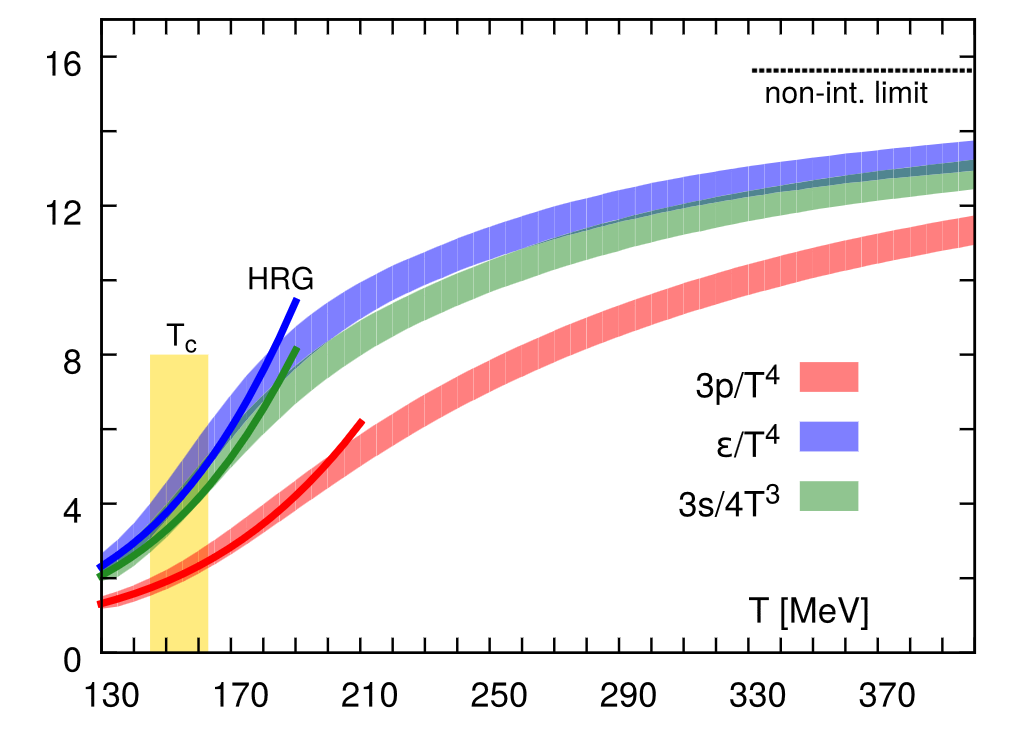
\includegraphics[width=.65\textwidth]{figures/normalized-thermo-quantities.pdf}
  \caption{Normalized thermodynamic quantities, showing the smooth-crossover transition and resulting increase in number of degrees of freedom.  Modified from \protect\cite{PhysRevD.90.094503}.}
  \label{fig:normalized-thermo-quantities}
\end{figure}


Note that in \ref{fig:normalized-thermo-quantities}, the measured thermodynamic quantites are compared against two limits: the low-temperature \gls{hrg} model, and the high-temperature Stefan-Boltzmann, ``non-interacting'' limit.
The \gls{hrg} limit
To explain the non-interacting limit, consider a non-interacting gas of gluons and quarks.
The energy density for such a system can be calculated by integrating the energy distributions and counting the allowed occupation number, i.e.
\begin{equation}
  \label{eqn:sb-energy-density}
  \varepsilon_{\text{SB}} = \int \frac{d^3p}{(2\pi)^3} \cdot p \left[ g^{\text{gluons}} n_{\text{B}}(p) + g^{\text{quarks}} n_{\text{F}}(p)  \right]
\end{equation}
where $n_{\text{B}}$ and $n_{\text{F}}$ are the Bose-Einsten and Fermi-Dirac momentum-space distributions, respectively, and the $g$ factors are the degeneracy factors (representing the number of degrees of freedom).
The distributions have the well known form
\begin{equation}
  n_{\text{B}}(p) = \frac{1}{e^{p/T} - 1} \ \ \ \ , \ \ \ \ n_{\text{F}}(p) = \frac{1}{e^{p/T} + 1}
\end{equation}
where we have ignored the chemical potential $\mu$ that would normally show up in $n_F$.
The degeneracy factors are
\begin{align}
  g^{\text{gluons}} &= \text{(spin states)} \times \text{(color states)} \\
  &= 2 \times 8 = 16 \notag
\end{align}
\begin{align}
  g^{\text{quarks}} &= \text{(spin states)} \times \text{(color states)} \times \text{(flavor states)} \times \text{(particle/anti-particle states)}\\
%  & \ \ \ \ \ \ \ \ \ \text{(particle/anti-particle states)} \notag \\
  &= 2 \times 3 \times 3 \times 2= 36 \notag
\end{align}
Thus \ref{eqn:sb-energy-density} becomes
\begin{align}
  \varepsilon_{\text{SB}} &= \frac{g^{\text{gluons}}}{\pi^2} \int dp \frac{p^3}{e^{p/T} - 1} + \frac{g^{\text{quarks}}}{\pi^2}\int dp \frac{p^3}{e^{p/T} + 1} \\
  &= \frac{g^{\text{gluons}}}{\pi^2} T^4 \int dp' \frac{p'^3}{e^{p'} - 1} + \frac{g^{\text{quarks}}}{\pi^2} T^4 \left(1 - \frac{1}{2^3}\right) \int dp' \frac{p'^3}{e^{p'} - 1}    \\ 
  &= \left( \frac{16}{\pi^2} + \frac{36}{\pi^2}\frac{7}{8} \right) \cdot \Gamma(4) \zeta(4) \cdot T^4 \\
  &= \frac{95 \pi^2}{60} T^4 \label{eqn:sb-energy-density-final-simple}
\end{align}
Therefore, the dashed line in \ref{fig:normalized-thermo-quantities} is a constant represented by the ratio from \ref{eqn:sb-energy-density-final-simple}.
The other plotted quantities also equal this constant due to the non-interacting relationship $\varepsilon_{\text{SB}} = 3 p_{\text{SB}} = \frac{3}{4} T s_{\text{SB}}$.
We note that the \gls{lqcd} simulation results remain about 20\% beneath this non-interacting limit.
The state-of-the-art \gls{lqcd} calculation of the critical temperature at $\mu_B = 0$ gives the value $T_c = (158.0 \pm 0.6)$ MeV \cite{PhysRevLett.125.052001}.

We have established via \gls{lqcd} that the $\mu_B = 0$ transition is a smooth crossover.
However, let us establish the other regions of the $T$ vs. $\mu_B$ phase-space -- i.e. the phase diagram of \gls{qcd}.
In the chiral limit of 2 massless quarks, the \gls{qcd} Lagrangian posseses chiral symmetry corresponding to SU(2)$_L$$\times$SU(2)$_R$.
However, due to the non-zero mass of the $u$ and $d$ quark, chiral symmetry is broken.
At high temperatures $T \gg \Lambda$ (i.e. in the \gls{qgp} phase), chiral symmetry is \textit{not} broken.
Thus there must be a phase boundary seperating nuclear matter from the deconfined \gls{qgp}.
Arguments based on the universality assert that the phase transition \textit{cannot} be second-order for massless quarks with $n_f = 3$ \cite{Stephanov:2006zvm}.
Thus, QCD with three massless quarks must undergo a first-order phase transition.

\begin{figure}[ht]
  \centering
  % Use .5\textwidth to only have the table fill half the page,
  % and \textwidth for the full page
  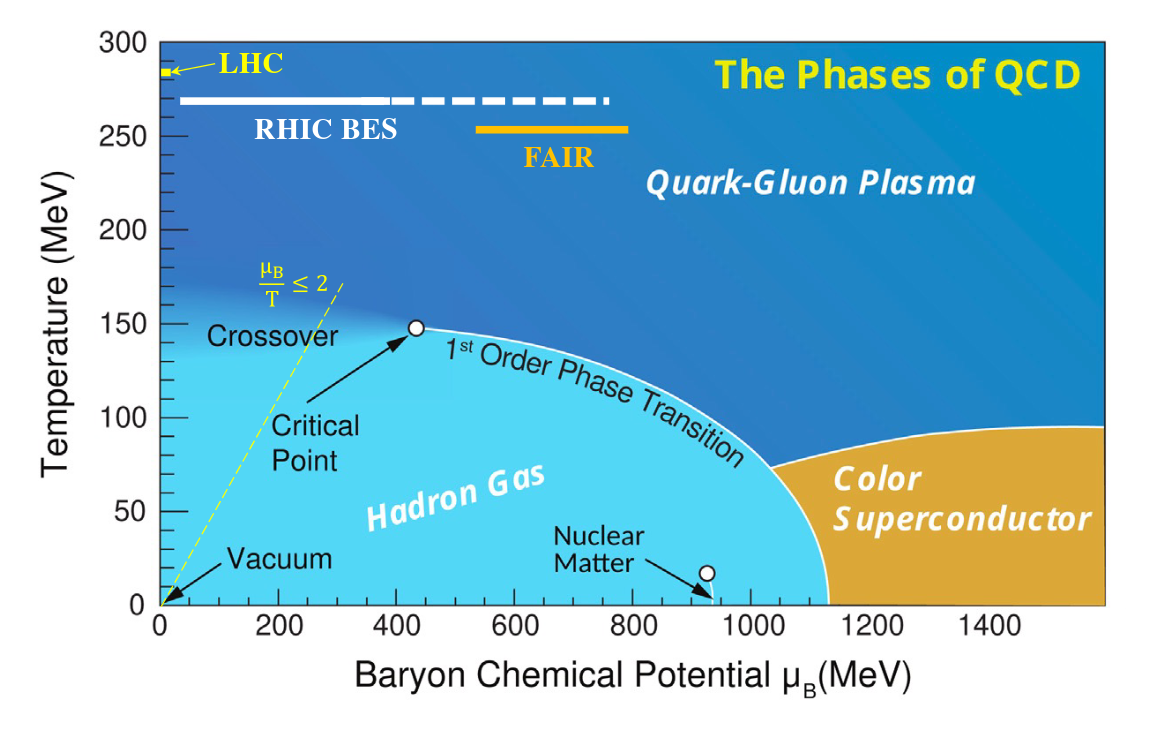
\includegraphics[width=.75\textwidth]{figures/qcd-phase-diagram.png}
  \caption{QCD phase diagram.  Figure from \protect\cite{Arslandok:2023utm}}
  \label{fig:qcd-phase-diagram}
\end{figure}


A modern interpretation of the QCD phase diagram is shown in \ref{fig:qcd-phase-diagram}.


